\documentclass[11pt, oneside, titlepage]{article}   	% use "amsart" instead of "article" for AMSLaTeX format
\usepackage{geometry}                		% See geometry.pdf to learn the layout options. There are lots.
\geometry{a4paper}                   		% ... or a4paper or a5paper or ... 
%\geometry{landscape}                		% Activate for rotated page geometry
\usepackage[parfill]{parskip}    			% Activate to begin paragraphs with an empty line rather than an indent
\usepackage{graphicx}				% Use pdf, png, jpg, or eps§ with pdflatex; use eps in DVI mode
								% TeX will automatically convert eps --> pdf in pdflatex		
\usepackage{amsthm, amsmath, amssymb}
\usepackage{float}

%SetFonts

%SetFonts


\title{Numerical Methods Coursework \\ \large{Group 10}\\}

\author{J.Waller E.Stables J.Gardner R.Tan S.Krishnamara F.Lau}
\date{4/3/18}							% Activate to display a given date or no date

\begin{document}
\maketitle

\section{RC Circuit}
\subsection{Exercise 1}
As expressed in the requirements, exercise 1 makes use of two functions, a RK2 which actually solves the differential equation, and RK2-script, which sets up the equations and provides calls to RK2. 

To simplify the results, the given equation has been rearranged in terms of $V_{out}$ ($V_r$):
\begin{equation}
\frac{1}{C}+Rq_C\text{'}(t)=V_{in}(t)
\end{equation}

\begin{equation}
V_{out}(t)=V_C(t)=\frac{1}{C}q_C(t)
\end{equation}

\begin{equation}
\Rightarrow CV_C(t)=q_C(t)
\end{equation}

\begin{equation}
\Rightarrow \frac{dq_C(t)}{dt}=C\frac{dV_C(t)}{dt
}\end{equation}

Substituting into the top equation gives:

\begin{equation}
RC\frac{dV_C(t)}{dt}=V_{in}(t)-\frac{1}{C}CV_C(t)
\end{equation}

\begin{equation}
\Rightarrow \frac{dV_{out}(t)}{dt}=\frac{1}{RC}(V_{in}(t)-V_{out}(t))
\end{equation}

Giving the final equation to be evaluated. Most of the stated questions have an initial condition of $V_{out}(t)=5V$. In some cases this is not the case (and it will be stated in these cases).

Physical Explanation: The behaviour of an RC circuit is reliant on the capacitor. A capacitor 'resists' changes in voltage over it, meaning an instant voltage change over it will be slowed to an exponential rise. This is due to the relationship between the voltage over a capacitor an the charge held within it, and the fact that a capacitor cannot output all of its charge in an instance:

$V_{C}C=Q$, showing the linear relationship between the charge (Q) and the voltage (VC). 
The reactance of a capacitor is determined by $Z_C=\frac{1}{j\omega C}$, showing that as the frequency increases, the reactance decreases. Therefore: $\lim_{\omega \to 0}=\infty$ showing that no current will flow in a DC circuit with a series capacitor. This implies that once the transients settle, there will be no voltage drops across any purely resistive components. All the voltage drop will be across the capacitor. 

Step Signals: The input step is formed with the matlab code:
\begin{verbatim}
Vin = @(t) 2.5*(t>=0)
\end{verbatim}

While the code Vin=5 would be correct, the equation in this form allows for an easy time shift if required. 
The output to this signal can be seen in figure \ref{fig:ex1_1}.

\begin{figure}[h]
\center
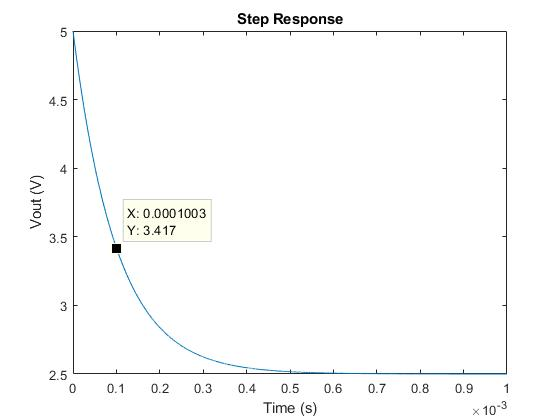
\includegraphics[scale = 0.5]{exercise1_1}
\caption{Step Response of RC Circuit} \label{fig:ex1_1}
\end{figure}




This clearly shows the initial condition exponentially decaying to the 2.5V input voltage. 

This circuit has $\tau = RC = 0.1\mu s$, indicating that a value should decrease by 63\%, with respect to its final value, within that timeframe. As can be seen on this plot, after $0.1\mu$s the output voltage has decreased from 5V to 3.417V, a decrease of 63.332\%.

Time shifting the step and expanding the time window shows the initial decrease and the rise. This demonstrates the rise and fall, both of them exponential and with the same characteristics.The output can be seen in figure \ref{fig:ex1_2}. 

\begin{figure}[H]
\center
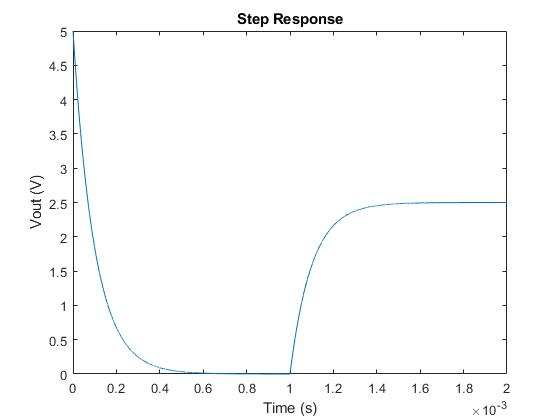
\includegraphics[scale = 0.5]{exercise1_2}
\caption{Step Response of RC Circuit} \label{fig:ex1_2}
\end{figure}

Finally, setting the value of the step to 5V shows the output remaining at a constant value, as there is never a point where the capacitor is required to discharge. This output can be seen in figure \ref{fig:ex1_3}

\begin{figure}[H]
\center
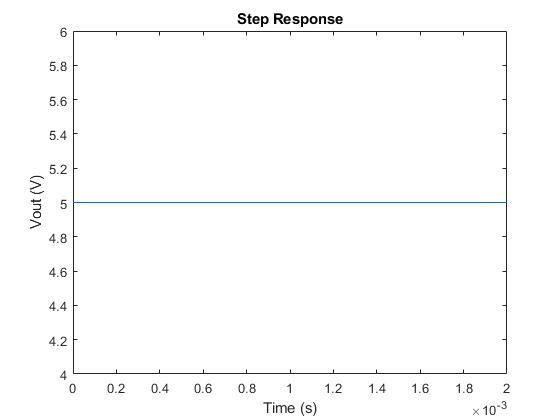
\includegraphics[scale = 0.5]{exercise1_3}
\caption{Step Response of RC Circuit} \label{fig:ex1_3}
\end{figure}

Time shifting this signal by $0.1\mu s$ shows the capacitor\text{'}s initial discharge, followed by it being charged back up by the stepped input. This output can be seen in figure \ref{fig:ex1_4}

\begin{figure}[H]
\center
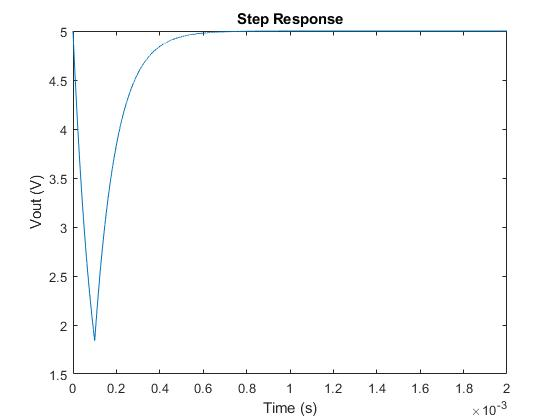
\includegraphics[scale = 0.5]{exercise1_4}
\caption{Step Response of RC Circuit} \label{fig:ex1_4}
\end{figure}

In this final case, the signal begins to drop from 5V towards 0V (as can be seen by the fact that $V_{out}$ has dropped to 1.85V at $0.1\mu s$, 37\% of 5V). However at $0.1\mu s$, when the step starts, the signal exponentially rises again. Again the time constant applies, at $0.2\mu s$ the voltage is 3.84V, which is 63\% of the rise from 1.85V to 5V. 


Impulse Signals: Two impulse signals were defined to be tested: 
\begin{equation}
V_{in}(t)=2.5exp(\frac{-t^2}{100(\mu s)^2})
\end{equation}

And:
\begin{equation}
V_{in}(t)=2.5exp(\frac{-t}{100\mu s})
\end{equation}

Both signals can be seen in figure \ref{fig:ex1_5}.

\begin{figure}[H]
\center
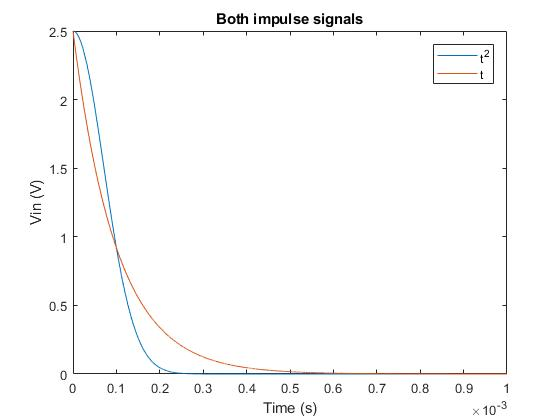
\includegraphics[scale = 0.5]{exercise1_5}
\caption{Both Input Signals} \label{fig:ex1_5}
\end{figure}

As can be seen, they are similar in magnitude, with the $t^2$ signal being held slightly longer, before dropping at an increased rate when compared to the signal linear in t. 

The response for the signal linear in $t$ can be seen in figure \ref{fig:ex1_6}

\begin{figure}[H]
\center
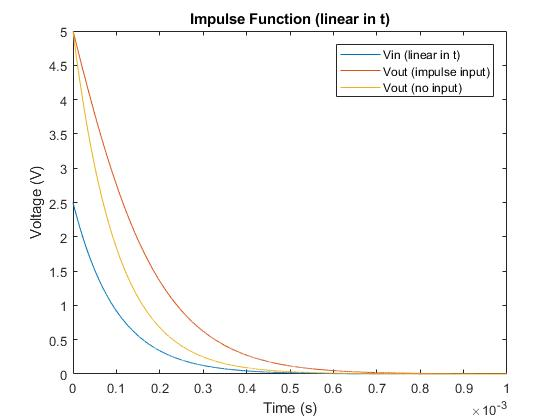
\includegraphics[scale = 0.5]{exercise1_6}
\caption{Impulse Linear in t} \label{fig:ex1_6}
\end{figure}

This plot shows the input function (blue), the output for the impulse input (red), and the normal output for the 5V initial condition but no input (yellow). As can be seen, the impulse output has a slower drop-off than the normal output. This can be explained as the extra voltage input puts a small voltage gradient across the capacitor, meaning that the output current from the capacitor is lower (as $I_C=C\frac{dV_C}{dt}$), and as $Q=\frac{dI}{dt}$ the lower current means that less charge is lost from the capacitor in the same amount of time. Therefore the voltage is kept at a higher level. 

With the initial condition removed the response can be seen in figure \ref{fig:ex1_7}

\begin{figure}[H]
\center
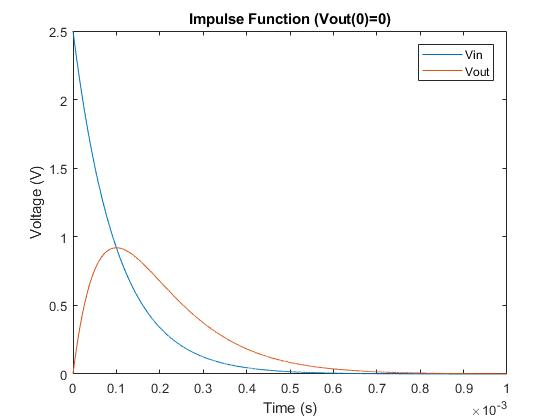
\includegraphics[scale = 0.5]{exercise1_7}
\caption{Impulse $V_{out}(0) = 0$} \label{fig:ex1_7}
\end{figure}

This shows how the voltage across the capacitor initially rises, until Vin matches, and drops below, Vout, Vout begins to drop again. However, we again see the capacitor 'resisting' the voltage drop, lagging the input voltage. Physically the behaviour can be explained by the equations $I_C=C\frac{dV_C}{dt}$ and $ I_C=\frac{V_{in}-V_C}{R}$ Initially $I_C$ is at a high value as $V_{in}$ is at its largest value, and $V_C$ is 0. This gives  $\frac{dV_C}{dt}$ a large initial value, giving $V_C$ an increasing value. As $V_C$ increases, and $V_{in}$ decreases, causing $I_C$ and therefore $\frac{dV_C}{dt}$ to also decrease. When $V_{in}=V_C$, $\frac{dV_C}{dt}=0$ and then becomes negative. This causes $V_{out}$ to rise, become constant while as it equals $V_{in}$, before decreasing.


Performing the same operations on the $t^2$ input:

\begin{figure}[H]
\center
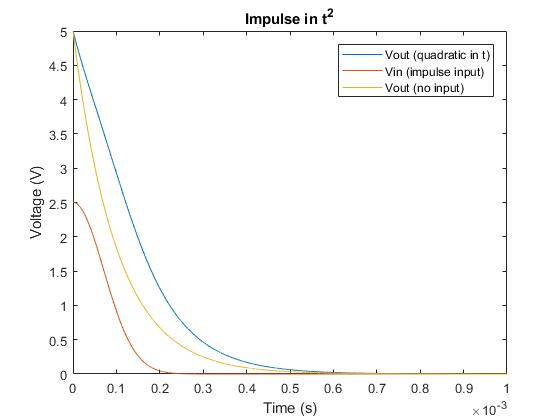
\includegraphics[scale = 0.5]{exercise1_8}
\caption{Impulse in $t^2$} \label{fig:ex1_8}
\end{figure}

Again with the linear impulse, the output seen in figure \ref{fig:ex1_8} is greater than the normal decline due to the reduced voltage across the capacitor, with a slower capacitor discharge.

\begin{figure}[H]
\center
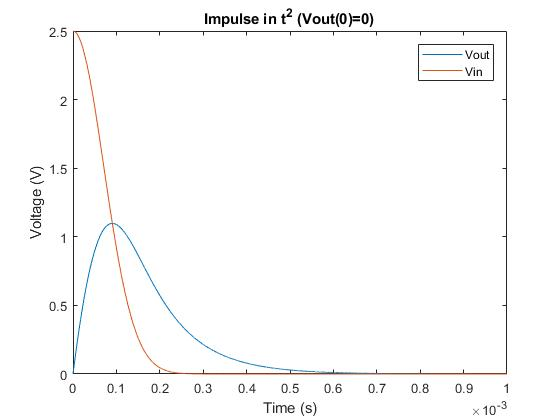
\includegraphics[scale = 0.5]{exercise1_9}
\caption{Impulse in $t^2$ $(V_{out}(0) = 0)$} \label{fig:ex1_9}
\end{figure}

Again, like the signal linear in t, the output seen in figure \ref{fig:ex1_9} can be seen to increase, until crossing to above the input voltage and dropping to 0.


\begin{figure}[H]
\center
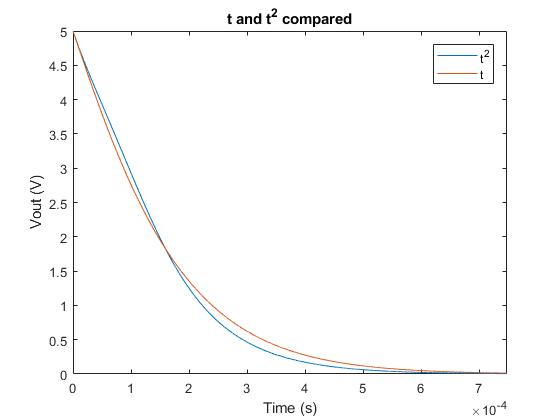
\includegraphics[scale = 0.5]{exercise1_10}
\caption{comparison of $t$ and $t^2$ output} \label{fig:ex1_10}
\end{figure}

Comparing the outputs (figure \ref{fig:ex1_10}) shows a very similar result, the signals decline at a similar rate, and become zero at approximately the same time. The difference in shape is the result of the $t^2$ equation, and the output plot mirrors the input plot. 

\begin{figure}[H]
\center
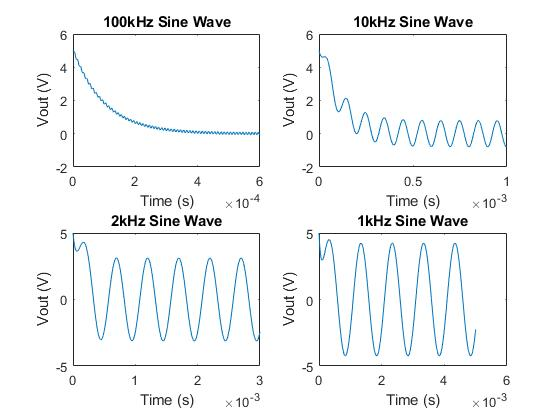
\includegraphics[scale = 0.5]{exercise1_11}
\caption{Sine Waves} \label{fig:ex1_11}
\end{figure}

Figure \ref{fig:ex1_11} shows the response of the system to sine waves at various frequencies. The shape of the signal is not distorted, once the initial transient has died down. It should also be noted that the signals with high frequency suffer a larger attenuation. The bode plot (figure \ref{fig:ex1_12}) of this network matches with the observed findings.

\begin{figure}[H]
\center
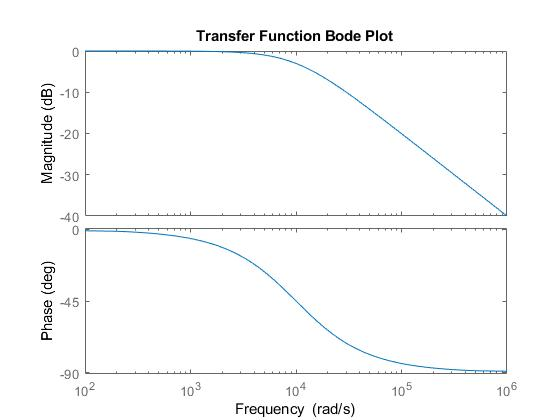
\includegraphics[scale = 0.5]{exercise1_12}
\caption{Transfer Function Bode Plot} \label{fig:ex1_12}
\end{figure}

It can also be observed that the higher frequency signals have a negative phase shift, although this is harder to observe. The steady state amplitudes of all the signals (in ascending frequency) are 0.09V,   0.79V, 3.113V, and 4.2V. Giving gains of -34.9dB, -16dB, -4.11dB, and -1.51dB respectively. These values can be seen to match up to the magnitude plot, with 628krad/s, 62.8krad/s, 12.57krad/s, and 6.28krad/s frequencies giving gains of -35dB, -15.1dB, -4.1dB,and -1.43dB. The inaccuracy is due to the resolution limitations of the bode plot. 

Figure \ref{fig:ex1_13} shows the square wave responses at various frequencies. As with the sine function, the magnitude of the square waves reduces at higher frequencies. However, this is not due to the attenuating features of the network. In this case, the capacitor is not allowing the voltage over it to change instantly, causing the curved increase seen in the 2kHz and 1kHz plots. As the output now takes time to reach its final value, as the signal increases in frequency, the output is not able to reach its final value before being forced to reduce again. The 1kHz signal reaches its final value just as it switches, however none of the other values are able to. 

\begin{figure}[H]
\center
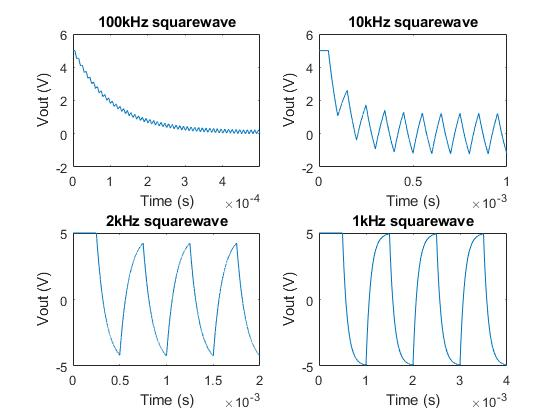
\includegraphics[scale = 0.5]{exercise1_13}
\caption{Square Waves} \label{fig:ex1_13}
\end{figure}

The steady 5V seen at the start of the 1kHz, 2kHz and 3kHz signals is a combination of the input signal and the initial condition. The input signal is at 5V, and if the capacitor was uncharged at the start then it would have the exponential rise seen in the other periods. However, the charged capacitor means that the signal will stay at a constant 5V until the input voltage is dropped, and the output must fall. 

In the case of the 100kHz signal (and partially the 10kHz one), a signal period is not enough time for the signal to fall into its normal periodic pattern. The signal reduces from the 5V initial value, but before it can fall all the way it has a small increase. However the constant positive voltage that is still across the output causes the falling voltage to always be larger than the rising voltage and the signal falls. Once the signal has a 0 average, there is no longer a positive bias over the capacitor, and the signal becomes periodic. 

\begin{figure}[H]
\center
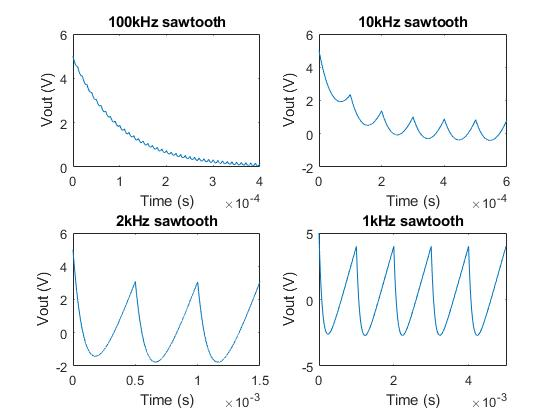
\includegraphics[scale = 0.5]{exercise1_14}
\caption{Sawtooth Waves} \label{fig:ex1_14}
\end{figure}

Figure \ref{fig:ex1_14} shows the sawtooth wave responses at various frequencies. Like the square wave, the sawtooth wave is attenuated as frequencies increase, with the same reason for the initial decline from 5V to a 0 average. The instant change from 5V to -5V becomes an exponential decrease (due to the discharging of the capacitor). As the input function instantly begins to rise again, the discharge of the capacitor does not behave as it would in a normal step, the increasing current through the capacitor slowing the discharge, and therefore the reduction in output voltage. Once the output voltage drops below the input voltage, it begins to charge again, increasing the output voltage at the same rate as the input voltage.  



Adjusting $\tau$:

The transient behaviour of the system is dependent on the time constant, $\tau$. Inputting a step response (with initial condition) at several values of $\tau$ demonstrates this, the outputs can be seen in figure \ref{fig:ex1_15}.

\begin{figure}[H]
\center
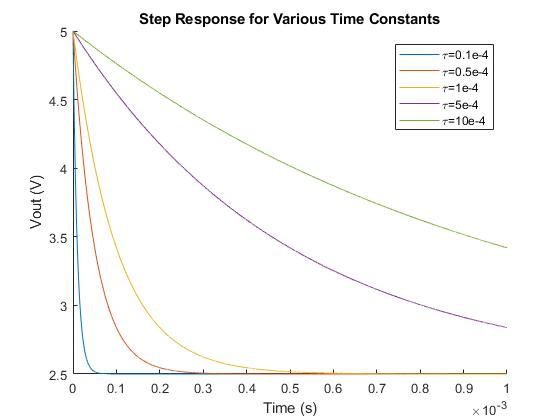
\includegraphics[scale = 0.5]{exercise1_15}
\caption{Step Response for Various Time Constants} \label{fig:ex1_15}
\end{figure}

As can be seen, the greater the value of $\tau$, the longer a signal takes to decrease. This can be explained by looking at the capacitor equation $\frac{I}{C} = \frac{dV_C}{dt}$ which may be written as $\frac{V_{in}-V_{out}}{RC} = \frac{dV_C}{dt}$, showing that the rate of change of the voltage is directly tied to the time constant $\tau = RC$, a larger RC causing a smaller rate of change, therefore taking longer to decrease. 




\subsection{Exercise 2}

The three numerical methods (Heun, Midpoint and Ralston) were used to approximate the solutions to first order ODE with different inputs. However, these numerical methods are only approximations and will therefore vary from the exact solution to the ODE. In this exercise, we will investigate the errors involved with each method by comparing the exact solutions to the solutions obtained by each method. 

To obtain the exact value we solve a first order ODE obtained through circuit analysis of the RC circuit with Initial condition given in exercise 1.

$V_{in} = 5V$, $\omega = 20k\pi rad/s$, $q = 500nC$, $R = 1000\Omega$, $C = 100nF$

\[R\frac{dq}{dt}+\frac{q}{C}=V_{in}\cos(\omega t) \]

\[\frac{dq}{dt}+\frac{q}{RC}=\frac{V_{in}}{R}\cos(\omega t) \]
\[Integrating factor =e^{\int\frac{1}{RC} dt} = e^{\frac{t}{RC}}\]
\[\frac{dq}{dt}e^{\frac{t}{RC}}+\frac{q}{RC}e^{\frac{t}{RC}}=\frac{V_{in}}{R}\cos(\omega t)e^{\frac{t}{RC}}\]
\[\frac{d}{dt}(qe^{\frac{t}{RC}})=\frac{V_{in}}{R}\cos(\omega t)e^{\frac{t}{RC}}\]
integrating both sides of the equation
\[qe^{\frac{t}{RC}}=\frac{V_{in}}{R}\int\cos(\omega t)e^{\frac{t}{RC}}dt\]
\[q=\frac{V_{in}C\cos(\omega t)+V_{in}\omega RC^2\sin(\omega t)+e^{\frac{-t}{RC}}(q(1+4\pi^2)-5V_{in}C)}{(1+(\omega RC)^2)}\]

The error function for each method is calculated by calling the function each method in RK2.m and then subtracting the approximation by the exact solution of the ODE.

\begin{figure}[H]
\center
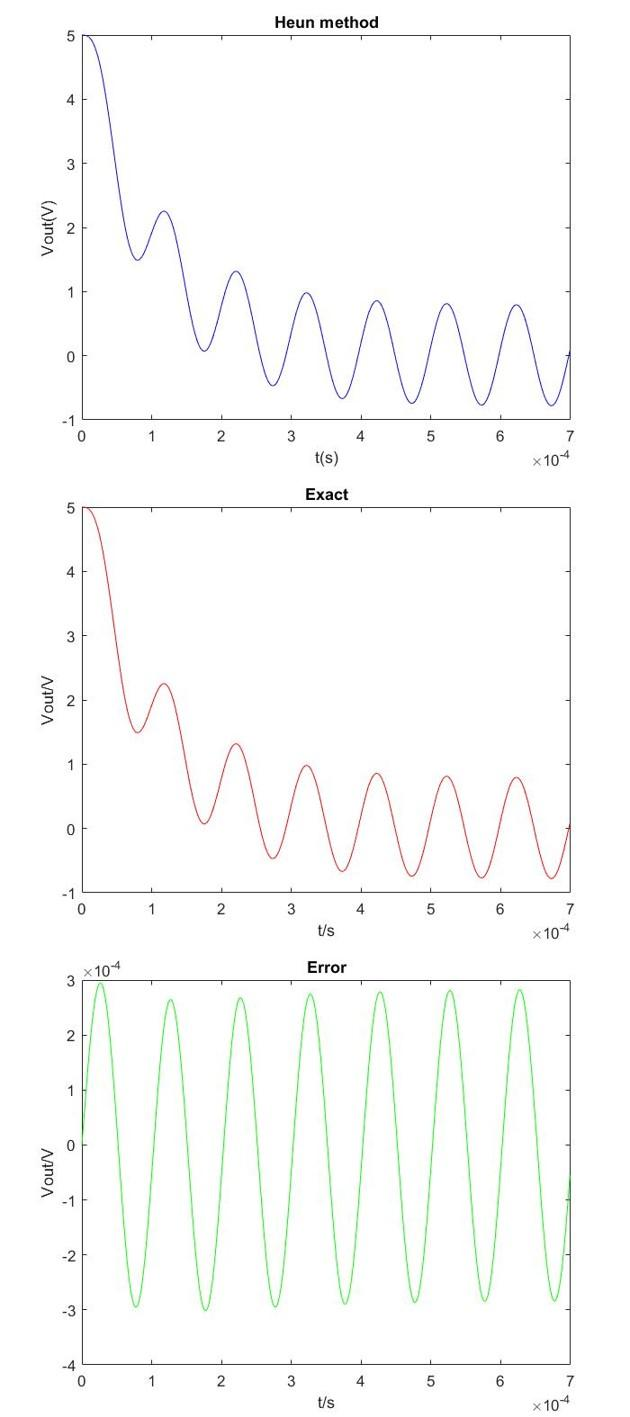
\includegraphics[scale = 0.35]{exercise2_1}
\caption{Error for Heun's Method} \label{fig:ex2_1}
\end{figure}

Figure \ref{fig:ex2_1} shows the solution and error generated using Heun's method. The first plot is the estimated solution using the Heun's method and this is then subtracted from the exact solution shown on the second plot to get the error plot. When the transient settles, the error oscillates with amplitude $2.81\times10^{-4}V$ and centre 0. Furthermore, it takes around $2.27\times10^{-4}s$ for the error to settle to 1\% of the steady state oscillation amplitude. For this method, the maximum error is $2.95\times10^{-4}V$ and this value is an overestimation since the error has a positive magnitude.

\begin{figure}[H]
\center
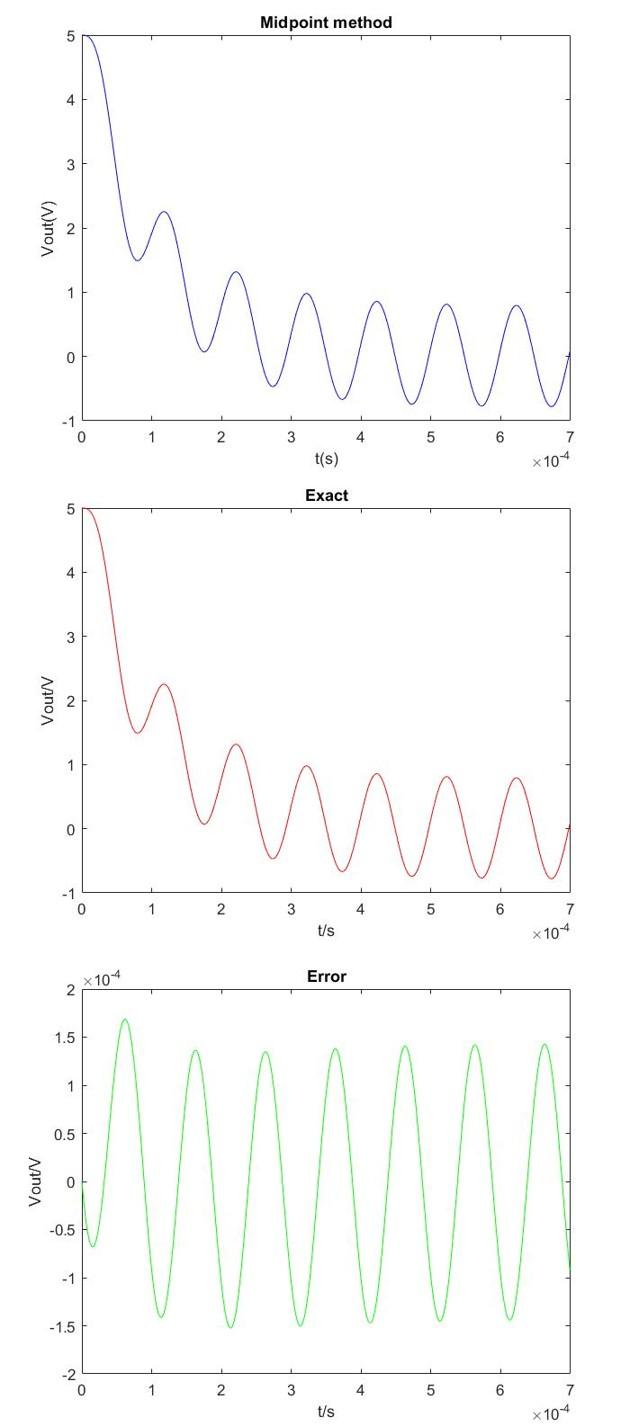
\includegraphics[scale = 0.35]{exercise2_2}
\caption{Error for Midpoint Method} \label{fig:ex2_2}
\end{figure}

Figure \ref{fig:ex2_2} shows the solution and error generated using Heun's method. The error function for the Midpoint method is calculated in the same way as for the Heun method since the exact solution is the same for all three methods. The first peak for the midpoint method is an underestimate since the magnitude of the amplitude is negative. However, the maximum error occurs after this peak, with an amplitude of $1.69\times10^{-4}V$. The transient then settles to less than 1\% of the steady state oscillation amplitude($1.42\times10^{-4}$V) after $4.63\times10^{-4}$s.

\begin{figure}[H]
\center
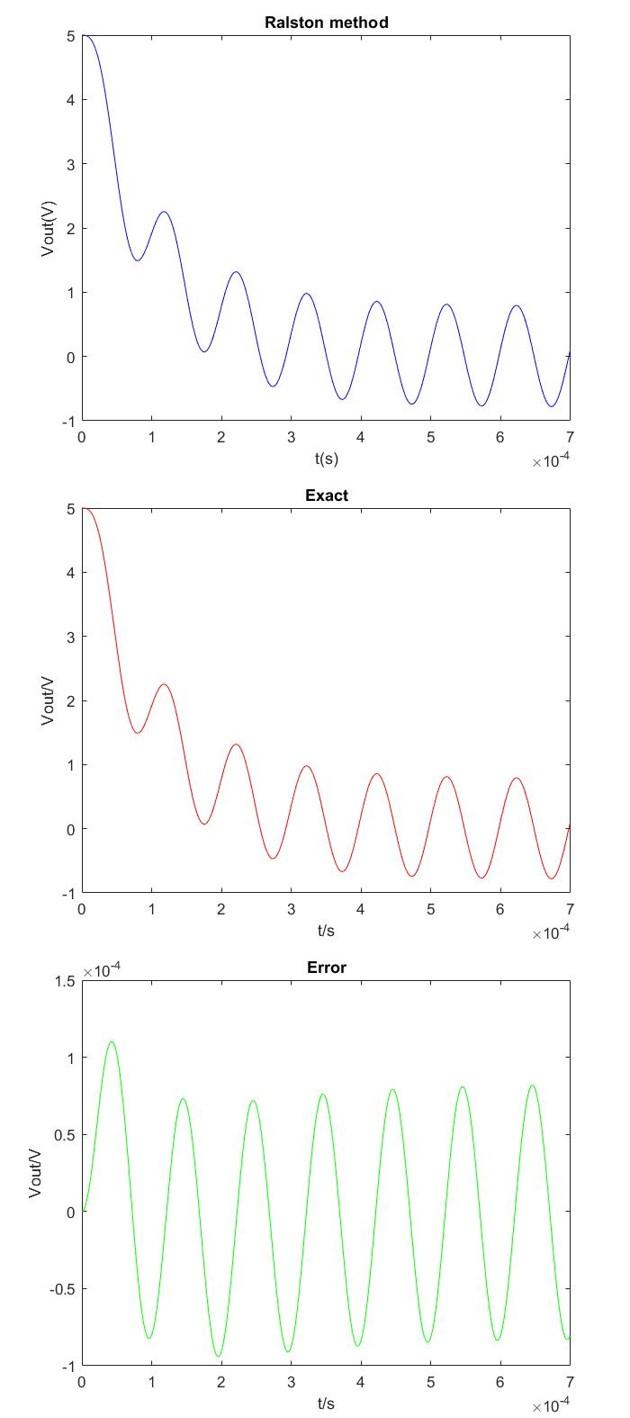
\includegraphics[scale = 0.35]{exercise2_3}
\caption{Error for Ralston Method} \label{fig:ex2_3}
\end{figure}

Figure \ref{fig:ex2_3} shows the solution and error generated using Ralston's method. The Ralston method also gives an oscillatory response which eventually settles to a steady state amplitude of $8.25\times10^{-5}$V. Before the steady state oscillations are achieved, the estimation to the Ralston method oscillate with offset from 0. It then takes take $8.45\times10^{-4}$s for the offset to become 0 and the error amplitude to settle to 1\% of the steady state amplitude. For this estimated solution, the maximum error is $1.10\times10^{-4}$V.

The analysis of the three methods above, shows that the error function is oscillatory after the transients have settled. However, the amplitude of oscillation for each method varies with the Heun's method having an amplitude of $2.812\times10^{-4}$V. The amplitude of the error function is reduced to $1.42\times10^{-4}$V by using the Midpoint method and the Ralston method has the smallest error with an amplitude of $8.25\times10^{-5}$V. Therefore, we can deduce that the Ralston method is the best method for approximating the solution to the given first order ODE. 

The error analysis was done by first creating an array of varying h from $10^{-5}$ to $10^{-8}$. Then each method numerical method was applied to solve the first order ODE and the error calculated for the corresponding step size. 

\begin{figure}[H]
\center
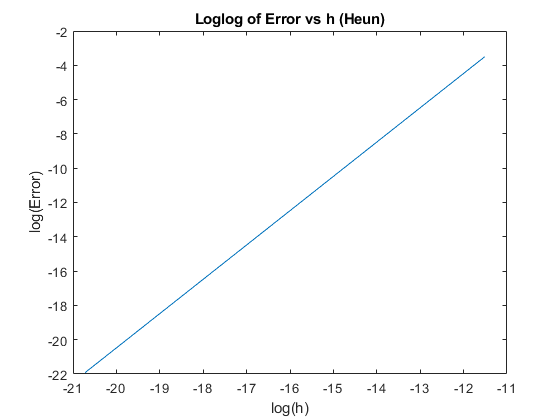
\includegraphics[width = 0.45\textwidth]{exercise2_4a}
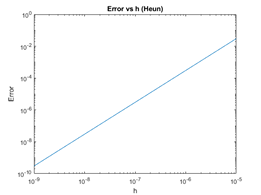
\includegraphics[width = 0.45\textwidth]{exercise2_4}
\caption{Log-Log Plots for Heun's Method} 
\end{figure}

\begin{figure}[H]
\center
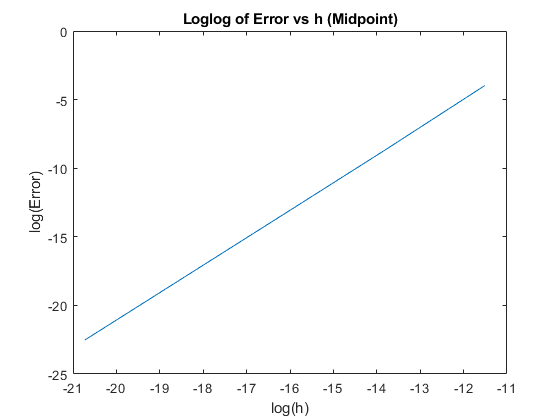
\includegraphics[width = 0.45\textwidth]{exercise2_5}
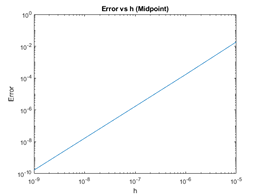
\includegraphics[width = 0.45\textwidth]{exercise2_5a}
\caption{Log-Log Plots for Midpoint Method} 
\end{figure}

\begin{figure}[H]
\center
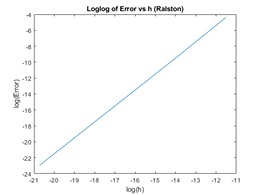
\includegraphics[width = 0.45\textwidth]{exercise2_6a}
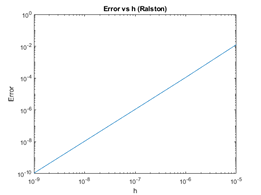
\includegraphics[width = 0.45\textwidth]{exercise2_6}
\caption{Log-Log Plots for Ralston Method}
\end{figure}

The plots show that there is a positive correlation between h and the error of the estimated solutions. By analysing the log-log plot of a method, We can find the order of the error.
The error function can be expressed as $log E = m log(h)+k$ 
By finding the gradient of the log-log plot, we can find the order of error. For the Heun method, the gradient is calculated to be 2.
\begin{equation}
log E=2log (h) + k
\end{equation}

Therefore $E(x,y)=O(h^2)$. The gradient of the straight line for the other two methods are also approximately 2, hence it can be concluded that the error is $O(h^2)$ for these second order RK methods.


\section{RLC Circuit}
RLC circuits are also known as resonant circuits, which behaves as a harmonic oscillator. We can use this circuit to select a particular range of frequencies, which is commonly called a band-pass filter.

\begin{figure}[H]
\center
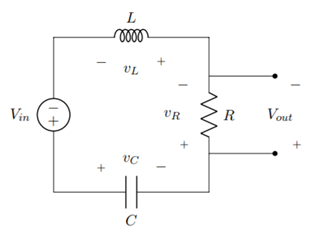
\includegraphics[scale = 0.5]{exercise3_1}
\caption{RLC Circuit} \label{fig:ex3_1}
\end{figure}

\subsection{Exercise 3}
We can derive expressions using the circuit above:
\begin{equation}
v_L(t)+v_R(t)+v_C(t)=V_{in}(t)
\end{equation}

Then, voltages of the components can be replaced by their respective parameters:
\begin{equation}
L\frac{di_L(t)}{dt}+Ri_L(t)+\frac{1}{C}\int_0^t{i_L(t)}=V_{in}(t)
\end{equation}

As $i(t)=\frac{dq}{dt}$ the equation can be rewritten as:
\begin{equation}
L\frac{d^2q_C(t)}{dt^2}+R\frac{dq_C(t)}{dt}+\frac{1}{C}q_C(t)=V_{in}(t)
\end{equation}

Input is Vin and output is $V_{out}=V_R=R\frac{dq_C(t)}{dt}$. Initial conditions are also given where: when t=0, capacitor is pre-charged at 500nC and no initial current flows through inductor so $i_L(0)=\frac{dq_C(0)}{dt}=0A$.

Values for respective components are: $R = 250\Omega$, $C = 3.5 \mu F$ and $L = 600 mH$.

RK4.m is a matlab function the implements the classic fourth-order Runge-Kutta for any system of two coupled first order equations:

\begin{equation}
z'=f_1(x,y,z) \text{ and } y'=f_2(x,y,z)
\end{equation}

Classic 4th Order Runge-Kutta Method:

\begin{equation}
k_1=f(x_i,y_i)
\end{equation}
\begin{equation}
k_2=f(x_i+0.5h,y_i+0.5k_1h)
\end{equation}
\begin{equation}
k_3=f(x_i+0.5h,y_i+0.5k_2h)
\end{equation}
\begin{equation}
k_4=f(x_i+h,y_i+k_3h)
\end{equation}
\begin{equation}
y_{i+1}=y_i+h(\frac{1}{6}k_1+\frac{1}{3}k_2+\frac{1}{3}k_3+\frac{1}{6}k_4)
\end{equation}

RLC-script.m is a matlab script which set up two coupled first order ODEs and calls RK4.m that solves the RLC second order ODE. The following shows the two coupled first order ODEs for the RLC circuit:

\begin{equation}z=y'\end{equation}
\begin{equation}z'=y''\end{equation}
\begin{equation}L\frac{di_L(t)}{dt}+Ri_L(t)+\frac{1}{C}\int_0^t{i_L(t)}=V_{in}(t)\end{equation}
\begin{equation}L\frac{d^2q_C(t)}{dt^2}+R\frac{dq_C(t)}{dt}+\frac{1}{C}q_C(t)=V_{in}(t)\end{equation}
\begin{equation}Lz'+Rz+\frac{1}{C}y=V_{in}(x)\end{equation}
\begin{equation}z'=\frac{1}{L}(V_{in}(x)-Rz-\frac{1}{C}y)\end{equation}
\begin{equation}y'=z\end{equation}

\begin{figure}[H]
\center
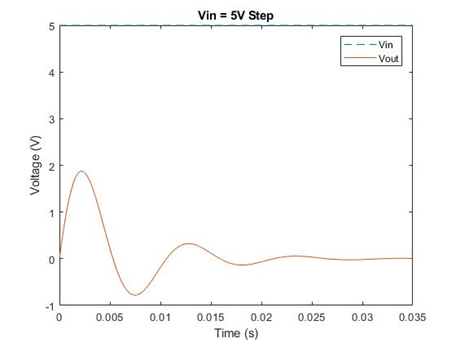
\includegraphics[scale = 0.5]{exercise3_2}
\caption{RLC with Step Input} \label{fig:ex3_2}
\end{figure}

Figure \ref{fig:ex3_2} shows the output of the RLC circuit when a step input it applied. As seen from the above plot, the transient response is affected by damping. Damping causes the decreasing amplitudes of the oscillations, which would ultimately make the output voltage=0. The higher the damping factor, the faster it is for the output voltage to approach zero. Damping factor is defined by $\zeta=\frac{R}{2}\sqrt{\frac{C}{L}}$. For this particular circuit, the damping factor is: $\zeta=\frac{R}{2}\sqrt{\frac{C}{L}}=\frac{250}{2}\sqrt{\frac{3.5*10^{-6}}{600*10^{-3}}}=0.3$. This indicates that oscillator is currently underdamped. 
The definition of damping factor suggests that if we increase the resistance, the damping factor would also increase by the same factor. To observe the output voltage of a higher damping factor, resistor value is now $1k\Omega$, then: $\zeta=\frac{1000}{2}\sqrt{\frac{3.5*10^{-6}}{600*10^{-3}}}=1.2$ 

With $R = 1k\Omega$, the oscillator is now overdamped. The peak is of a higher magnitude, because we are now using a higher resistance, so potential difference is going to be larger.

\begin{figure}[H]
\center
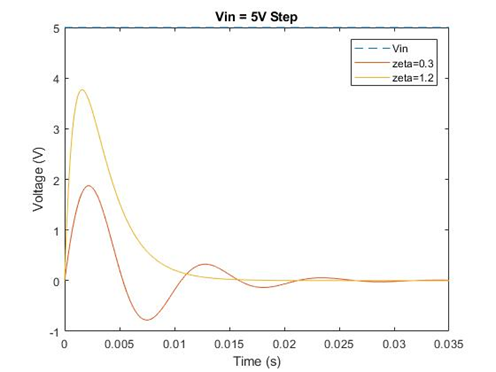
\includegraphics[scale = 0.5]{exercise3_3}
\caption{RLC with Step Input, Overdamped} \label{fig:ex3_3}
\end{figure}

\begin{figure}[H]
\center
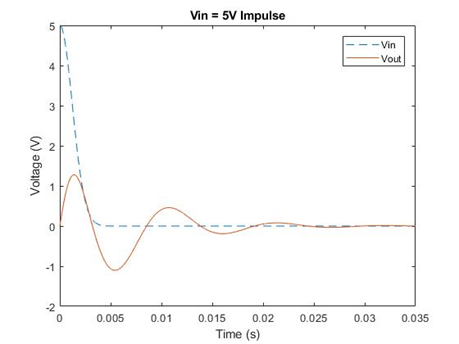
\includegraphics[scale = 0.5]{exercise3_4}
\caption{RLC with Impulse Input} \label{fig:ex3_4}
\end{figure}

Figure \ref{fig:ex3_4} shows the output of the RLC circuit when an impulse is applied. The plot is very similar to the previous plot (step signal). For both scenarios, 5V is applied as soon as t becomes zero, and both oscillate at a decreasing amplitude until they become zero. A notable difference will be the magnitude, it is observed that the impulsive signal with decay has a much lower magnitude than the step response and this is due to the impact of $exp(-\frac{t^2}{\tau})$. It is therefore concluded that the impulse response is influenced by the decay instead of damping because the transient decreases as soon as the decay took place, yet the oscillation cannot stop completely after the decay happens, so oscillation continues until it becomes zero. To prove this, a simulation of impulsive signal was done again but this time with $\tau = 12 (ms)^2$:

\begin{figure}[H]
\center
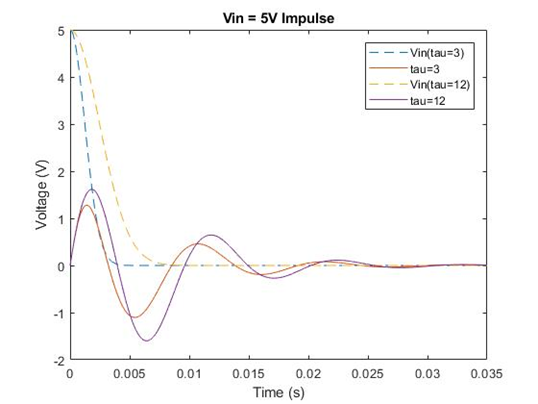
\includegraphics[scale = 0.5]{exercise3_5}
\caption{RLC with Impulse Input, larger $\tau$} \label{fig:ex3_5}
\end{figure}

Figure \ref{fig:ex3_5} shows that with a bigger tau, the decay took place later compared to the original plot. The output voltage with a bigger tau also drops slightly later compared to the original plot as expected. 

\begin{figure}[H]
\center
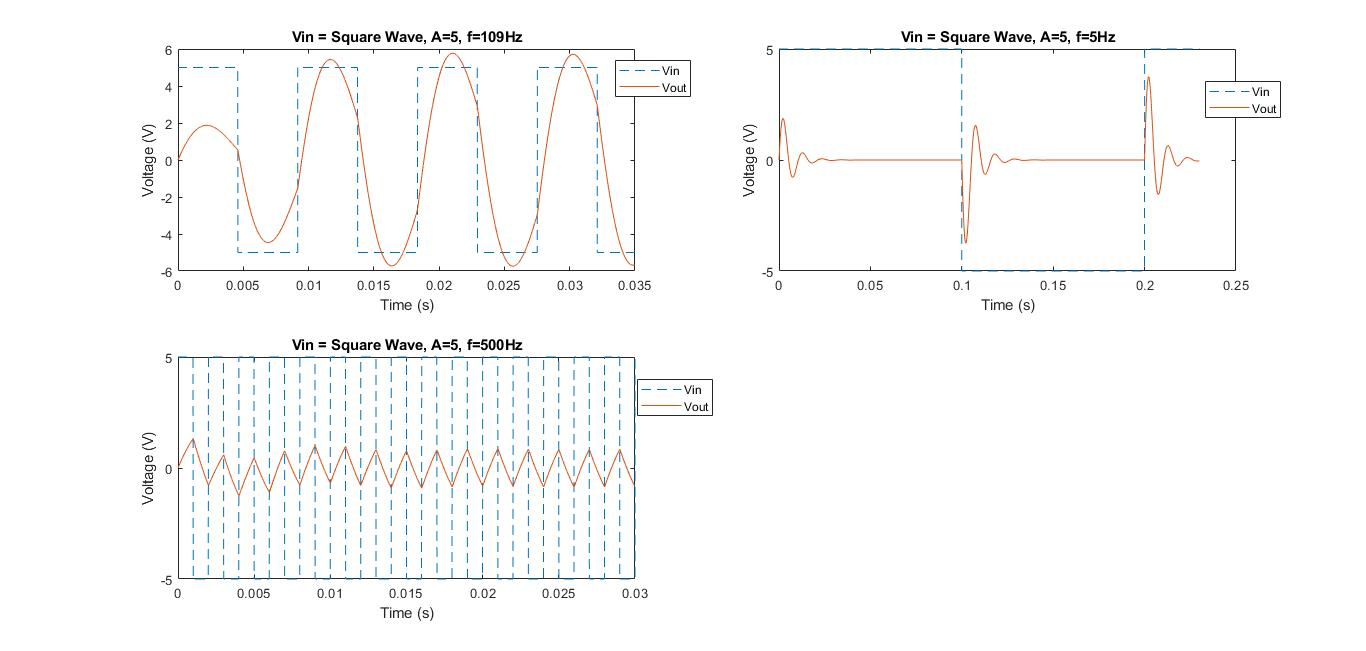
\includegraphics[scale = 0.35]{exercise3_6}
\caption{RLC Square Wave Response} \label{fig:ex3_6}
\end{figure}

The square wave response (figure \ref{fig:ex3_6}) shows several behaviours of the circuit. As the output is taken over the resistor, the steady state DC value will always remain 0. This is due to the fact that the capacitor offers an infinite impedance to purely DC terms, meaning that no current flows and therefore no voltage can be dropped across the resistor. 
At 5Hz each discontinuity causes a spike before settling to 0V. This behaviour is identical to the behaviour of the step response, with the negative going transition causing the inverse response.

The square wave can be treated as a series of discontinuities, as it is in the 5Hz example. It can be seen that partway along each rise and fall of each period there is a small 'kink' in the signal. This is when the input has a discontinuity, shown as the time between each kink is 9.21ms, and the period of the signal is 9.17ms, with the small difference being due to the lack of resolution on the plot. Inspection of the response after each discontinuity and comparing it to the step response shows that the signal is the same. The oscillations in the 5Hz plots shows the impact of damping on the system as shown in earlier plots of this exercise. When the frequency of the square wave is 109Hz, which is the resonant frequency of the RLC ciruict, the oscillations are no longer forced and the gain of the system is one. Therefore, the peaks of input square wave and output sinusoidal wave are very similar in magnitude.

\begin{equation}
\omega_c = \frac{1}{2\pi \sqrt{LC}} = \frac{1}{2\pi \sqrt{600\times10^{-3}\times3.5\times10^{-6}}} = 109Hz
\end{equation}

The  500Hz signal has a similar behaviour to the previous signal, in that each discontinuity can be treated as a step response. However, the higher frequency means that the next discontinuity occurs before much of the response can be seen, giving the signal the appearance of a triangle wave. It is worth noting that the amplitude is vastly reduced compared to the input signal due to the discontinuities occuring before the signal can approach the input value.

\begin{figure}[H]
\center
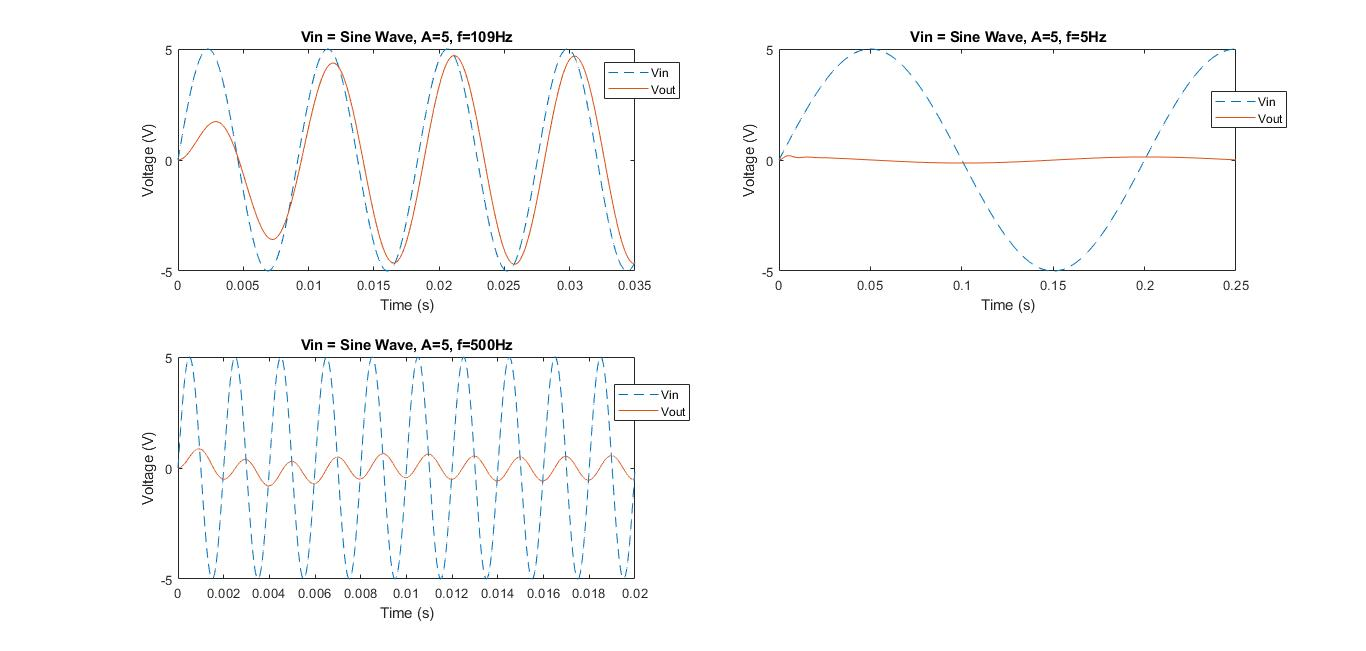
\includegraphics[scale = 0.35]{exercise3_7}
\caption{RLC Sine Wave Response} \label{fig:ex3_7}
\end{figure}

We can observe from all output voltages that they are all sinusoidal wave, which is one of the characteristics of sinusoidal waves, that the waveform does not change even after integration or differentiation. Therefore, only smooth changes in voltage is observed unlike the plots for square waves at different frequencies. In addition, unlike all the other signals in this exercise, input voltage does not change abruptly, which is another reason for the smooth changes. Damping effect is not significant in any of the plots above. It is observed from all 3 plots that phase is shifted in the output voltage.

When frequency is 109Hz, which is its resonant frequency, the gain would be 1, therefore the magnitude of peaks are almost identical, giving an almost identical waveform if the phase shift and the first peak is ignored. When frequency is at 5Hz and 500Hz, magnitude of the amplitude is a lot less than the input signal, as both frequencies are both far away from resonant frequency (109Hz) in different directions. 

As mentioned before, the first cycle of the output sinusoidal waves should be ignored as it does not match with the rest of the waveform. The first cycle shows the response of the RLC circuit from a sudden increase in voltage applied, slowing climbing to the peak observed later. On the other hand, the first cycle of the wave at 5Hz shows a slightly different waveform from the other first cycles of other frequencies:

\begin{figure}[H]
\center
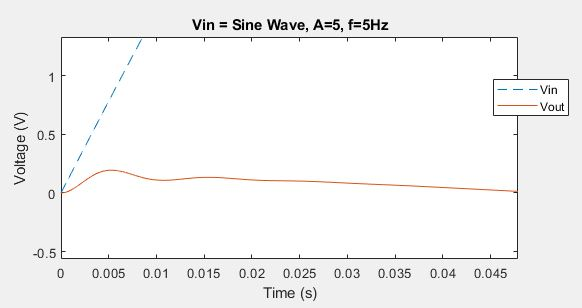
\includegraphics[scale = 0.5]{exercise3_8}
\caption{RLC Sine Wave Response 5Hz} \label{fig:ex3_8}
\end{figure}

This behaviour was seen from the step and impulse response, which damping is affecting the waveform.



\section{Relaxation}
\subsection{Exercise 4}

Created Script relaxation1.m which implements the relaxation method to solve Laplace's equation on the unit square. Laplace's equation is:

\begin{equation}
\frac{\partial^2u}{\partial x} + \frac{\partial^2u}{\partial y} = 0
\end{equation}

Which can be approximated as:

\begin{equation}
\frac{u(x+h, y) - 2u(x, y) + u(x-h, y)}{h^2} + \frac{u(x, y+h) -2u(x, y) + u(x, y-h)}{h^2} = 0
\end{equation}

on a grid with known boundaries, where $h$ is the length of the side of each square on the grid. Using this method allows us to approximate each point as the mean of its 4 adjacent points:

\begin{equation}
U_i^j = \frac{U_{i+1}^j + U_{i-1}^j + U_i^{j+1} + U_i^{j-1}}{4}
\end{equation}

This equation allows us to iterate through the grid and calculate a better approximation for each point every time. In order to test for convergence, the residue is defined as:

\begin{equation}
r^j_i = (U_i^j)_{new} - (U_i^j)_{old}
\end{equation}

Where $(U_i^j)_{new}$ is the mean value of the points adjacent to $U_i^j$ and $(U_i^j)_{old}$ is the current value of $U_i^j$. The residue gets smaller with every pass though the grid and the program stops after the maximum value of the residue in the grid is smaller than the desired accuracy $r_{max}$.

If the boundary conditions are known, this method can be used. Initially as the interior points of the grid are not known, they will be set to the mean value of the boundary conditions.


Initial boundary conditions:
$\phi_1 = 0$, 
$\phi_2 = 0$, 
$\phi_3 = 
\begin{cases}	1, & 0.2 \leq x \leq 0.8 \\
			0, & \text{otherwise}  \end{cases}$, 
$\phi_4 = 0$ 
 

Using a step size of 0.02 and a maximum residue of 0.0001 gives the output shown in figure \ref{fig:relaxation1}.

\begin{figure}[H]
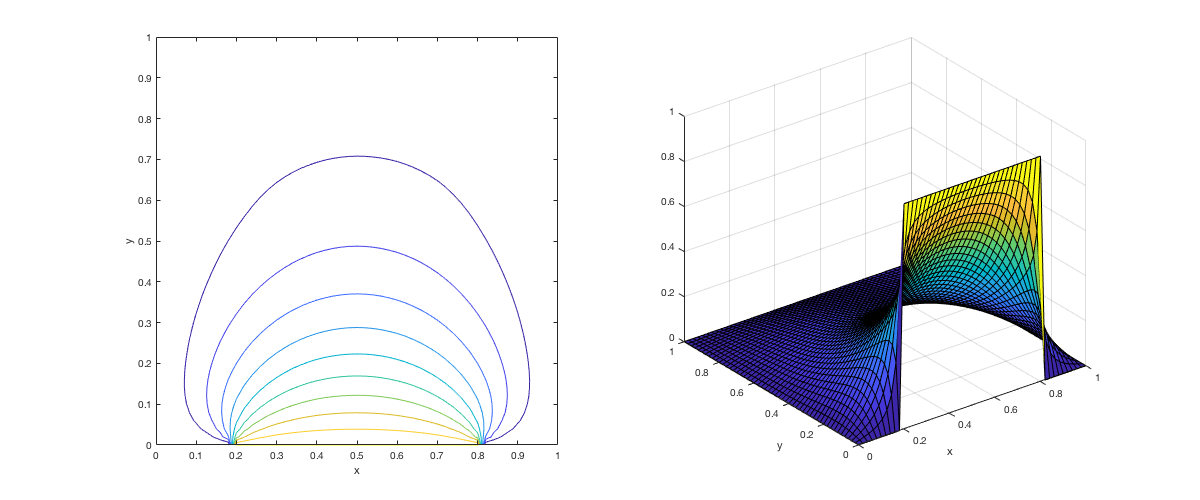
\includegraphics[width = \textwidth]{relaxation1_1}
\caption{Solution with given boundary conditions} \label{fig:relaxation1}
\end{figure}


Using a larger residue (0.001) means some of the values of the array remain unchanged from the initial value (mean of the boundary conditions) which were put in initially. This is shown in figure \ref{fig:relaxation1a}.

\begin{figure}[H]
	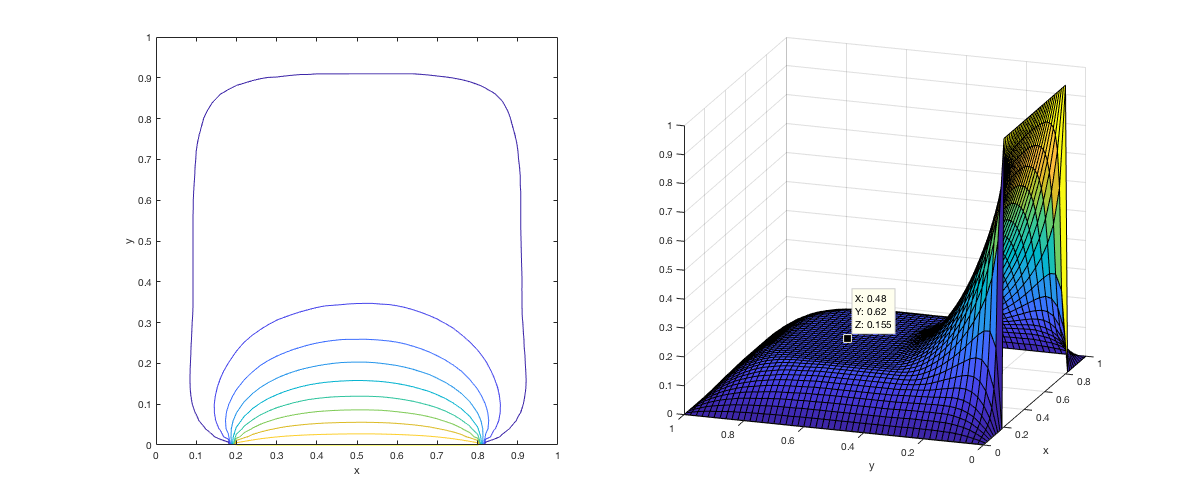
\includegraphics[width = \textwidth]{relaxation1_1a}
	\caption{Solution with given boundary conditions, $r_{max} = 0.001$} \label{fig:relaxation1a}
\end{figure}

The residue can be set to zero, in which case it will go down to the accuracy of the floating point arithmetic MATLAB uses. This solution is shown in figure \ref{fig:relaxation1b}.

\begin{figure}[H]
	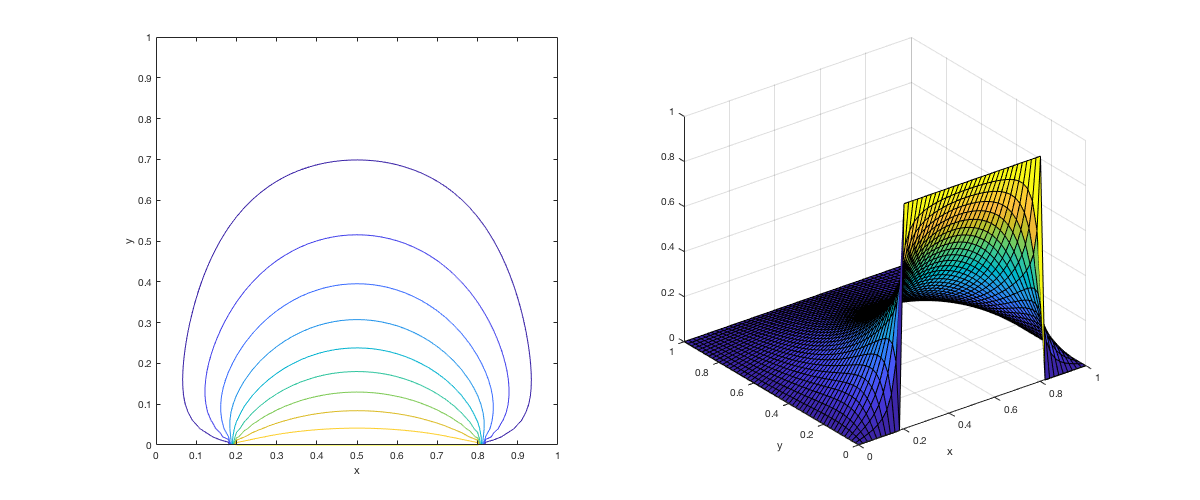
\includegraphics[width = \textwidth]{relaxation1_1b}
	\caption{Solution with given boundary conditions, $r_{max} = 0$} \label{fig:relaxation1b}
\end{figure}

Changing the gridsize by decreasing h increases the running time of the program, as the new value of U and the residue have to be evaluated at more points per loop.  Decreasing the residue also increases the running time of the program, as the program has to loop more times in order for every value to be less than $r_{max}$.


The second set of boundary conditions: $\phi_1 = -sin(x\pi)$, $\phi_2 = sin(y\pi)$, $\phi_3 = -sin(x\pi)$, $\phi_4 = sin(y\pi)$ give 'saddle'  shape with equipotentials $y = x$ and $y = 1-x$. This is shown in figure \ref{fig:relaxation12}.

\begin{figure}[H]
	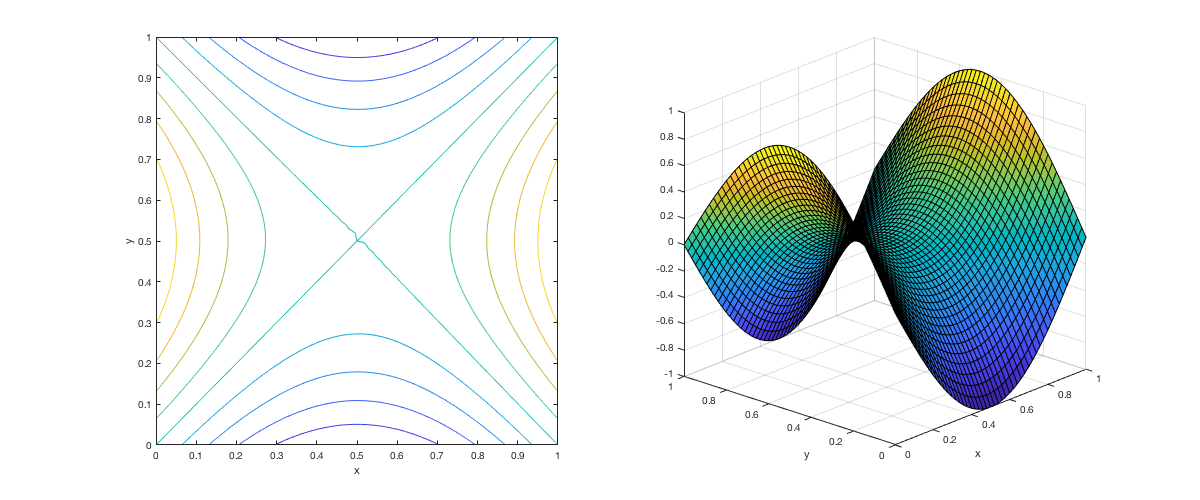
\includegraphics[width = \textwidth]{relaxation1_2}
	\caption{Solution with second boundary conditions, $r_{max} = 0.0001$} \label{fig:relaxation12}
\end{figure}

The final set of boundary conditions: $\phi_1 = 0$, $\phi_2 = 0$, $\phi_3 = 1$, $\phi_4 = 0$ have a discontinuity at $(0,0)$ and at $(1,0)$ as shown in figure \ref{fig:relaxation1c}. At these points the value of U cannot be multiple values, so the point must be chosen to be equal to one of the boundary conditions. In this case $U(0,0) = 0$ and $U(1,0) = 0$, as the way the program is written the boundaries $\phi_2$ and $\phi_4$ will overwrite the corners with their value when the program starts. This is only a problem at large h where the gradient between the corner and the next point on the boundary with the correct value would be noticeable, but for sufficiently small h the effect is minimised, and the discontinuity remains.

\begin{figure}[H]
	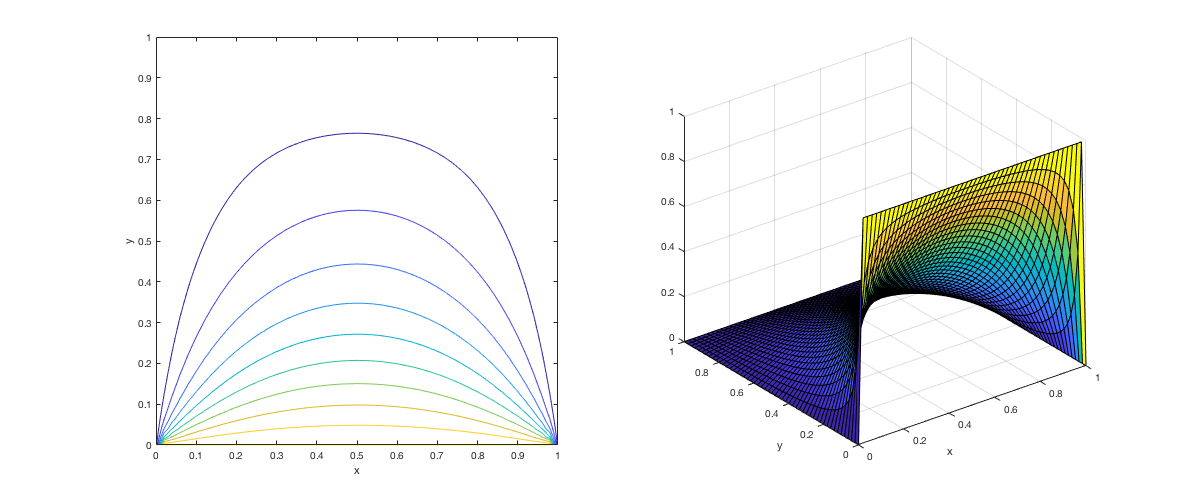
\includegraphics[width = \textwidth]{relaxation1_1c}
	\caption{Solution with third boundary conditions} \label{fig:relaxation1c}
\end{figure}

\subsection{Exercise 5}

Created Script relaxation2.m which implements the relaxation method to solve Poisson's equation on the unit square. Poisson's equation is:

\begin{equation}
\frac{\partial^2u}{\partial x} + \frac{\partial^2u}{\partial y} = g(x,y)
\end{equation}

Which can be approximated as:

\begin{equation}
\frac{u(x+h, y) - 2u(x, y) + u(x-h, y)}{h^2} + \frac{u(x, y+h) -2u(x, y) + u(x, y-h)}{h^2} = g(x,y)
\end{equation}

on a grid with known boundaries, where $h$ is the length of the side of each square on the grid. Using this method allows us to approximate each point as the mean of its 4 adjacent points:

\begin{equation}
U_i^j = \frac{U_{i+1}^j + U_{i-1}^j + U_i^{j+1} + U_i^{j-1} - g_i^jh^2}{4}
\end{equation}

The residual is the same as is used for Laplace's equation:

\begin{equation}
r^j_i = (U_i^j)_{new} - (U_i^j)_{old}
\end{equation}

In this case the solution to Poisson's equation is:

\begin{equation}
u(x,y) = 2x^2 +y^2 + x -2xy
\end{equation} 

Poisson's equation then becomes:

\begin{equation}
\frac{\partial^2u}{\partial x} + \frac{\partial^2u}{\partial y} = 6
\end{equation}

The boundary conditions for this function are: $\phi_1 = 2x^2 - x + 1$, $\phi_2 = y^2 -2y +3$, $\phi_3 = 2x^2 +x$, $\phi_4 = y^2$.

Using a gridsize of 0.01 and a residue of 0.00001 gives the figure \ref{fig:ex5_1} as outputs. The error (figure \ref{fig:ex5_1a}) plot is obtained by subtracting the values obtained by the relaxation method from the exact solution and then plotting. As you can see, the maximum error is 0.0101. 

\begin{figure}[H]
	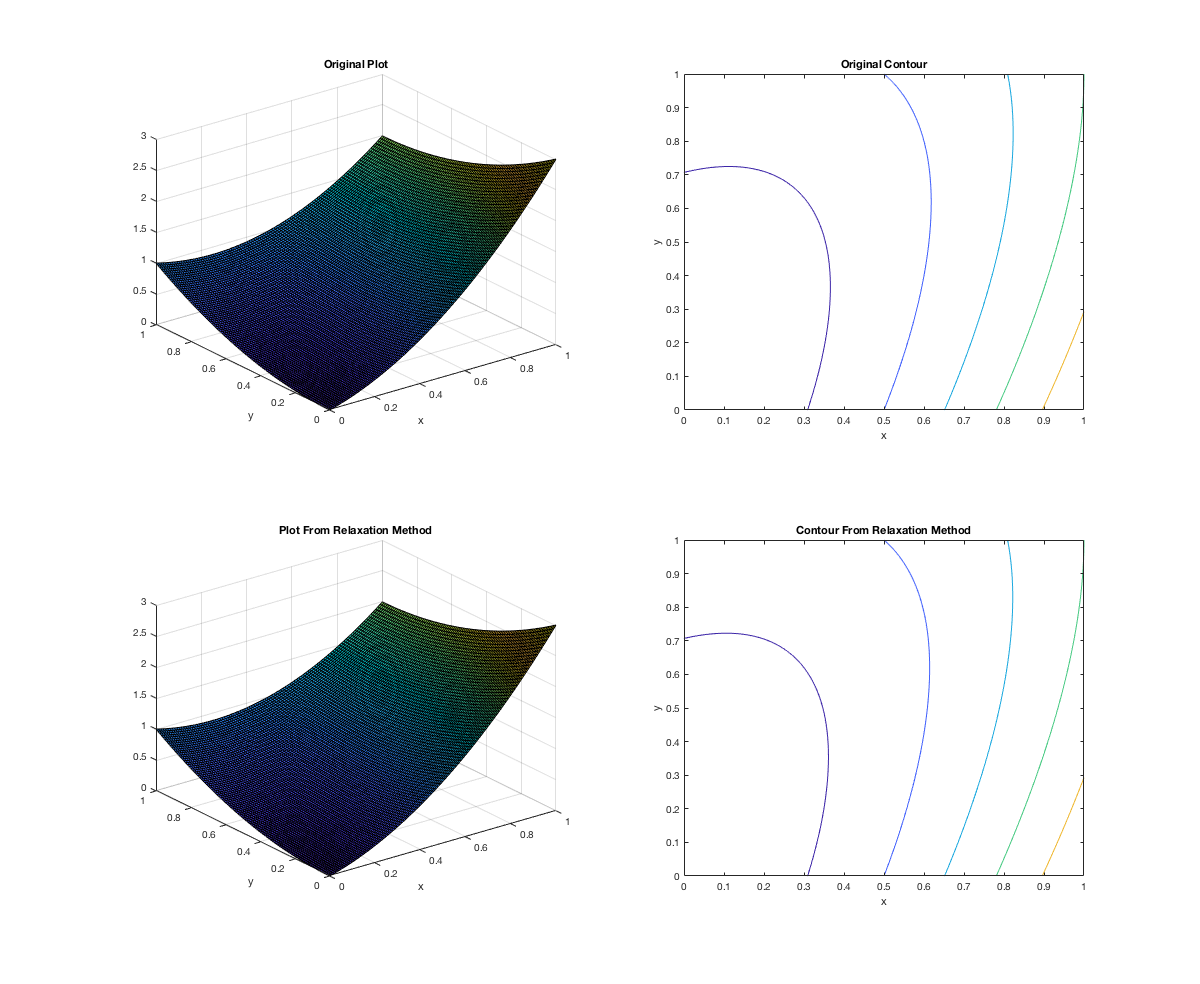
\includegraphics[width = \textwidth]{exercise5_1}
	\caption{Relaxation Method for Poisson's Equation} \label{fig:ex5_1}
\end{figure}

\begin{figure}[H]
	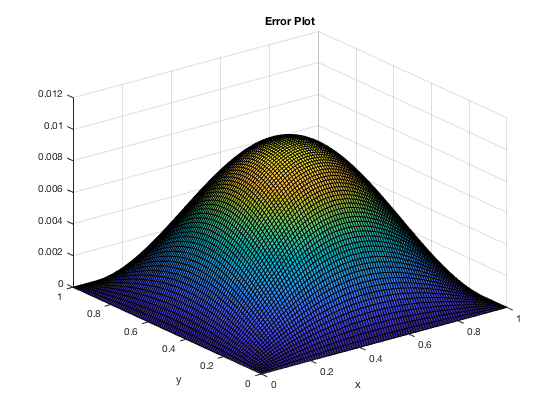
\includegraphics[width = \textwidth]{exercise5_1a}
	\caption{Error in Relaxation Method for Poisson's Equation} \label{fig:ex5_1a}
\end{figure}

relaxation2.m was then tested to find the order of the error based on the residue. It was tested for residue in the range [0,0.01] with the errors shown in figure \ref{fig:ex5_2}  as you can see, the error varies from $2.953\times10^-14$ to $1.301$ (the error is not zero when residue equals zero due to the accuracy of the floating point arithmetic MATLAB uses).

\begin{figure}[H]
	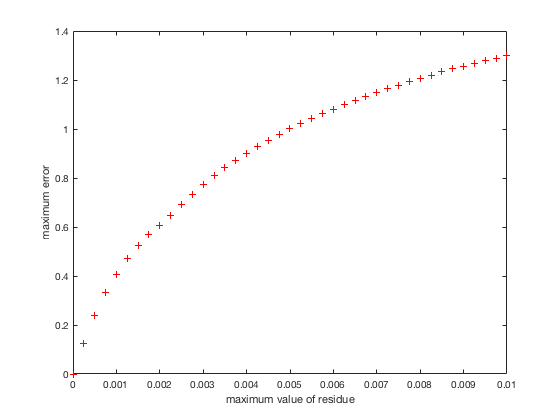
\includegraphics[width = \textwidth]{exercise5_2}
	\caption{Error in Relaxation Method for Different Residues} \label{fig:ex5_2}
\end{figure}

From this it can be concluded that the error caused by the residue is approximatley $O(\sqrt{r})$

\subsection{Optional Successive Over Relaxation}

For Successive over-relaxation method the residue calculation is changed to include the over-relaxation parameter $s$:

\[r_i^j=s\frac{U_{i+1}^j+U_{i-1}^j+U_{i}^{j+1}+U_{i}^{j-1}-4U_i^j}{4}\]

The value of $s$ will depend on the problem being solved and may vary as the iteration process converges. However, in these particular examples, a value of 1.4 produces good results. The number of times which the while loop runs decreases from 7939 to 3477 for relaxation1.m.
 
After implementing SOR, the iteration time for the while loop also decreases from 30758 to 13281 
In some special cases it is possible to determine an optimal value analytically using the equation as follows:

\[s=\frac{2}{1+\frac{\pi}{n}}\]

\begin{figure}[H]
	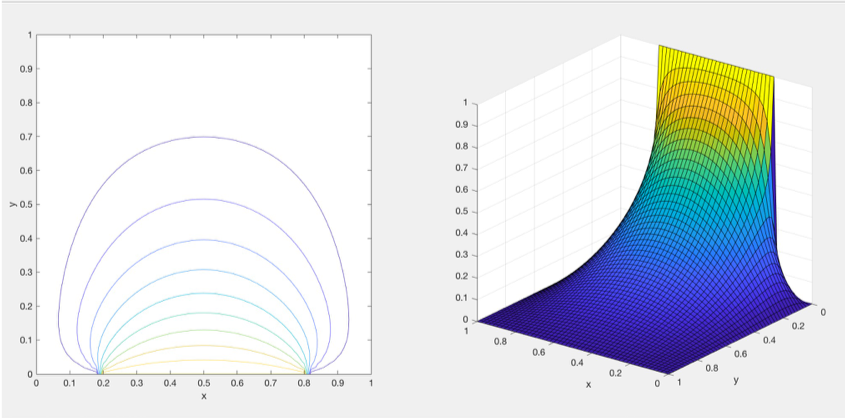
\includegraphics[width = \textwidth]{SOR_1}
	\caption{relaxation1.m using SOR} \label{fig:SOR_1}
\end{figure}

\begin{figure}[H]
	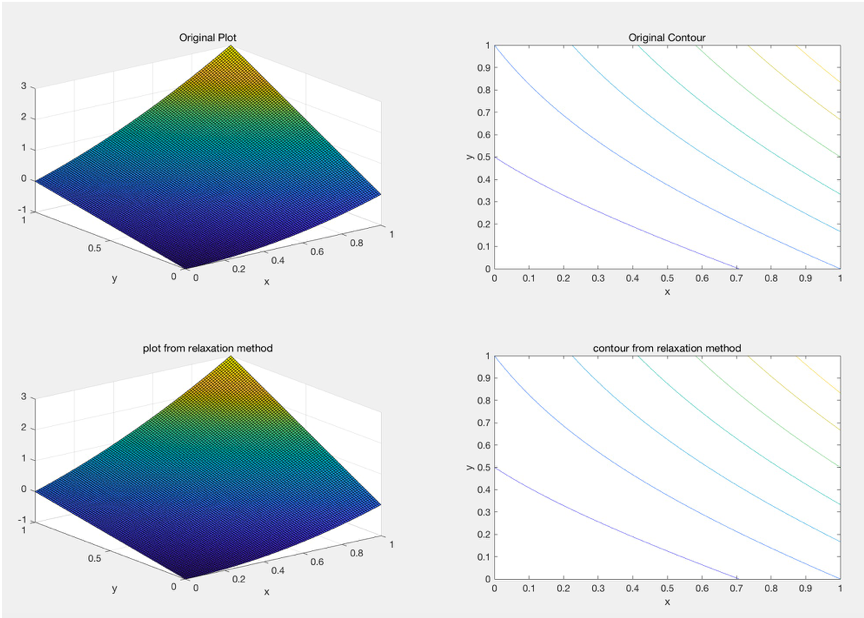
\includegraphics[width = \textwidth]{SOR_2}
	\caption{relaxation2.m using SOR} \label{fig:SOR_2}
\end{figure}

\begin{figure}[H]
	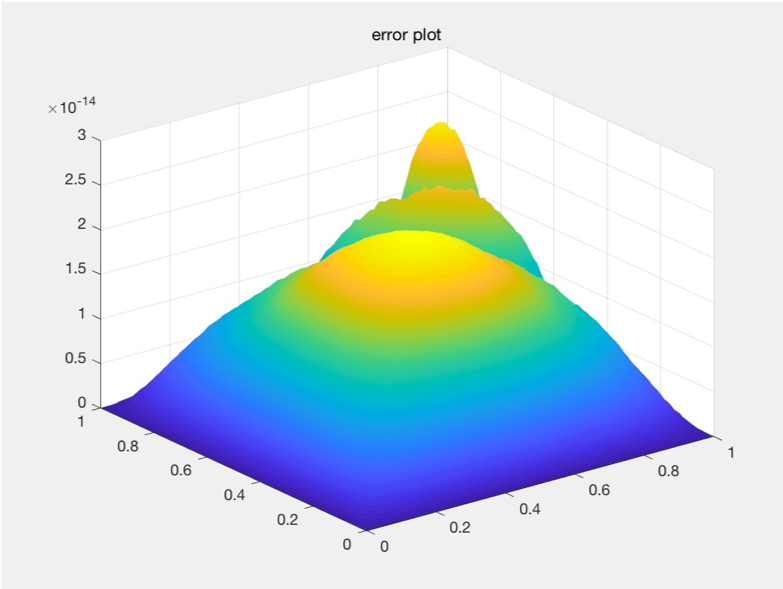
\includegraphics[width = \textwidth]{SOR_3}
	\caption{relaxation2.m error plot using SOR} \label{fig:SOR_3}
\end{figure}


\end{document}  